\documentclass[1p]{elsarticle_modified}
%\bibliographystyle{elsarticle-num}

%\usepackage[colorlinks]{hyperref}
%\usepackage{abbrmath_seonhwa} %\Abb, \Ascr, \Acal ,\Abf, \Afrak
\usepackage{amsfonts}
\usepackage{amssymb}
\usepackage{amsmath}
\usepackage{amsthm}
\usepackage{scalefnt}
\usepackage{amsbsy}
\usepackage{kotex}
\usepackage{caption}
\usepackage{subfig}
\usepackage{color}
\usepackage{graphicx}
\usepackage{xcolor} %% white, black, red, green, blue, cyan, magenta, yellow
\usepackage{float}
\usepackage{setspace}
\usepackage{hyperref}

\usepackage{tikz}
\usetikzlibrary{arrows}

\usepackage{multirow}
\usepackage{array} % fixed length table
\usepackage{hhline}

%%%%%%%%%%%%%%%%%%%%%
\makeatletter
\renewcommand*\env@matrix[1][\arraystretch]{%
	\edef\arraystretch{#1}%
	\hskip -\arraycolsep
	\let\@ifnextchar\new@ifnextchar
	\array{*\c@MaxMatrixCols c}}
\makeatother %https://tex.stackexchange.com/questions/14071/how-can-i-increase-the-line-spacing-in-a-matrix
%%%%%%%%%%%%%%%

\usepackage[normalem]{ulem}

\newcommand{\msout}[1]{\ifmmode\text{\sout{\ensuremath{#1}}}\else\sout{#1}\fi}
%SOURCE: \msout is \stkout macro in https://tex.stackexchange.com/questions/20609/strikeout-in-math-mode

\newcommand{\cancel}[1]{
	\ifmmode
	{\color{red}\msout{#1}}
	\else
	{\color{red}\sout{#1}}
	\fi
}

\newcommand{\add}[1]{
	{\color{blue}\uwave{#1}}
}

\newcommand{\replace}[2]{
	\ifmmode
	{\color{red}\msout{#1}}{\color{blue}\uwave{#2}}
	\else
	{\color{red}\sout{#1}}{\color{blue}\uwave{#2}}
	\fi
}

\newcommand{\Sol}{\mathcal{S}} %segment
\newcommand{\D}{D} %diagram
\newcommand{\A}{\mathcal{A}} %arc


%%%%%%%%%%%%%%%%%%%%%%%%%%%%%5 test

\def\sl{\operatorname{\textup{SL}}(2,\Cbb)}
\def\psl{\operatorname{\textup{PSL}}(2,\Cbb)}
\def\quan{\mkern 1mu \triangleright \mkern 1mu}

\theoremstyle{definition}
\newtheorem{thm}{Theorem}[section]
\newtheorem{prop}[thm]{Proposition}
\newtheorem{lem}[thm]{Lemma}
\newtheorem{ques}[thm]{Question}
\newtheorem{cor}[thm]{Corollary}
\newtheorem{defn}[thm]{Definition}
\newtheorem{exam}[thm]{Example}
\newtheorem{rmk}[thm]{Remark}
\newtheorem{alg}[thm]{Algorithm}

\newcommand{\I}{\sqrt{-1}}
\begin{document}

%\begin{frontmatter}
%
%\title{Boundary parabolic representations of knots up to 8 crossings}
%
%%% Group authors per affiliation:
%\author{Yunhi Cho} 
%\address{Department of Mathematics, University of Seoul, Seoul, Korea}
%\ead{yhcho@uos.ac.kr}
%
%
%\author{Seonhwa Kim} %\fnref{s_kim}}
%\address{Center for Geometry and Physics, Institute for Basic Science, Pohang, 37673, Korea}
%\ead{ryeona17@ibs.re.kr}
%
%\author{Hyuk Kim}
%\address{Department of Mathematical Sciences, Seoul National University, Seoul 08826, Korea}
%\ead{hyukkim@snu.ac.kr}
%
%\author{Seokbeom Yoon}
%\address{Department of Mathematical Sciences, Seoul National University, Seoul, 08826,  Korea}
%\ead{sbyoon15@snu.ac.kr}
%
%\begin{abstract}
%We find all boundary parabolic representation of knots up to 8 crossings.
%
%\end{abstract}
%\begin{keyword}
%    \MSC[2010] 57M25 
%\end{keyword}
%
%\end{frontmatter}

%\linenumbers
%\tableofcontents
%
\newcommand\colored[1]{\textcolor{white}{\rule[-0.35ex]{0.8em}{1.4ex}}\kern-0.8em\color{red} #1}%
%\newcommand\colored[1]{\textcolor{white}{ #1}\kern-2.17ex	\textcolor{white}{ #1}\kern-1.81ex	\textcolor{white}{ #1}\kern-2.15ex\color{red}#1	}

{\Large $\underline{12n_{0760}~(K12n_{0760})}$}

\setlength{\tabcolsep}{10pt}
\renewcommand{\arraystretch}{1.6}
\vspace{1cm}\begin{tabular}{m{100pt}>{\centering\arraybackslash}m{274pt}}
\multirow{5}{120pt}{
	\centering
	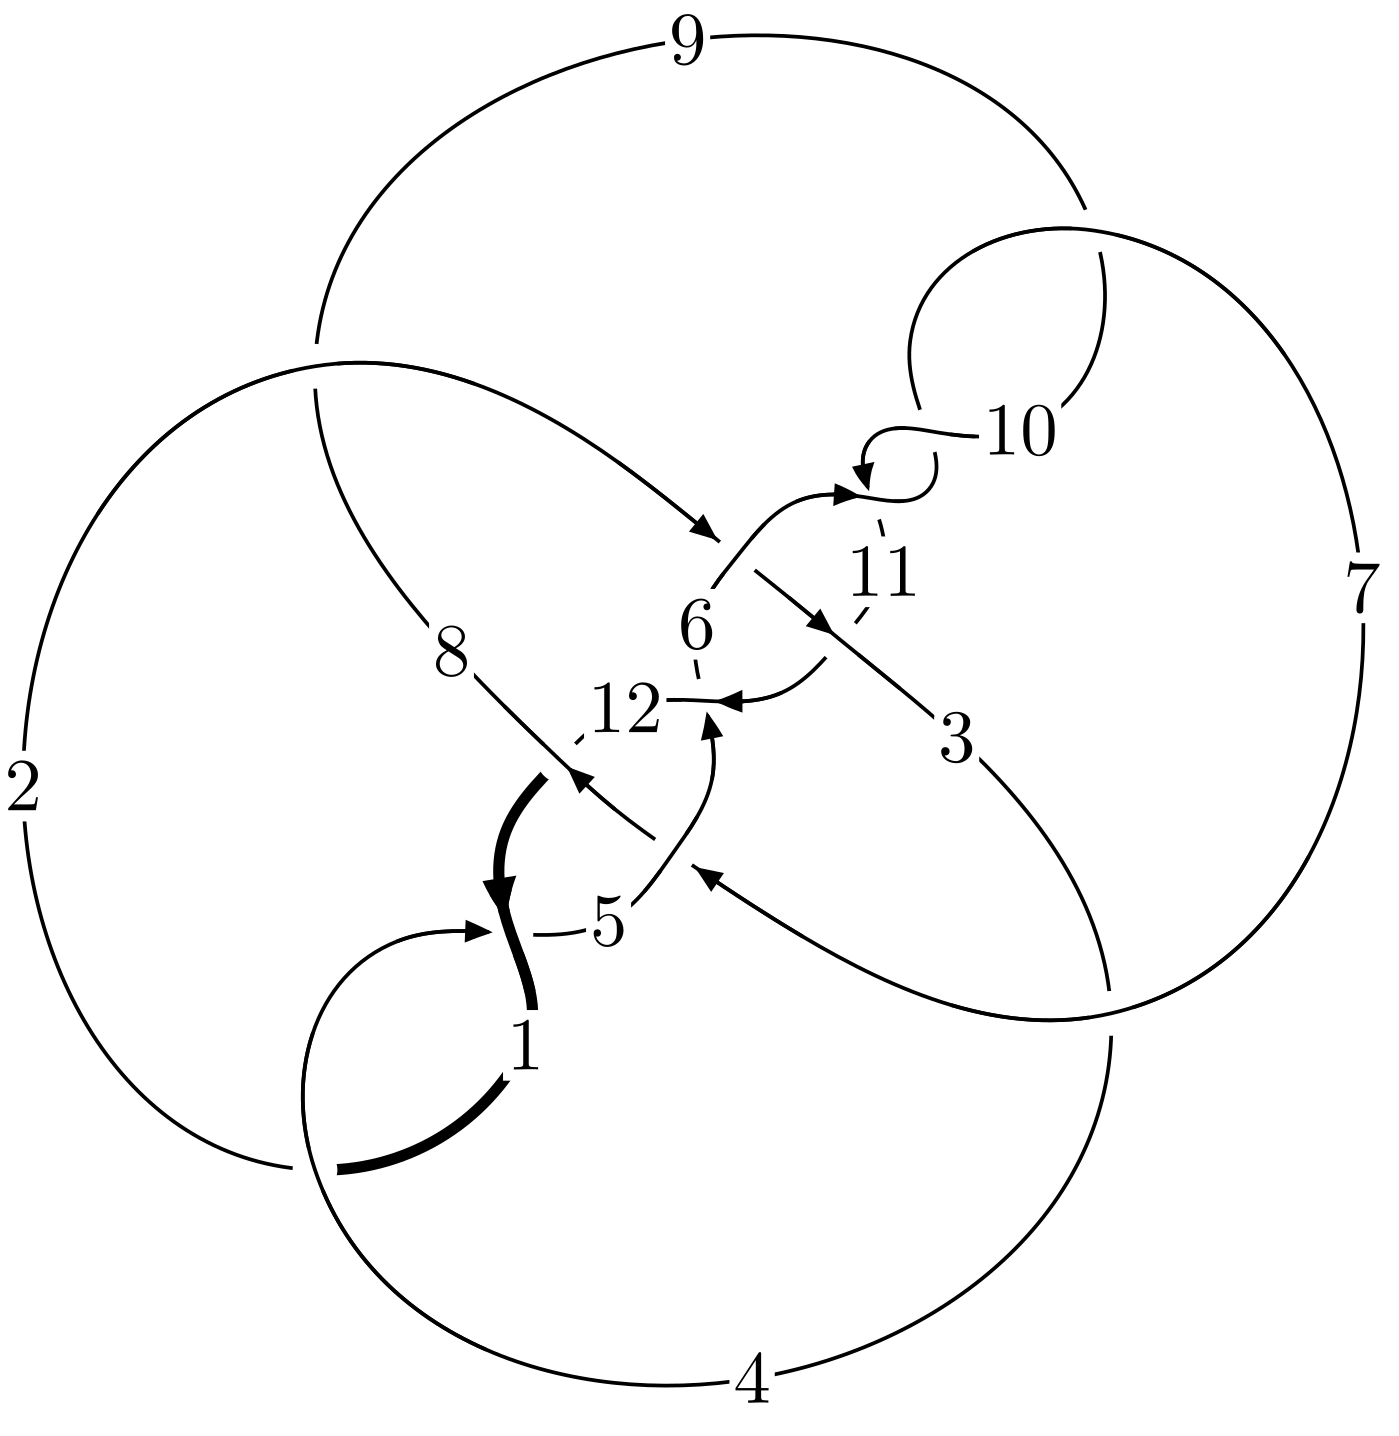
\includegraphics[width=112pt]{../../../GIT/diagram.site/Diagrams/png/2849_12n_0760.png}\\
\ \ \ A knot diagram\footnotemark}&
\allowdisplaybreaks
\textbf{Linearized knot diagam} \\
\cline{2-2}
 &
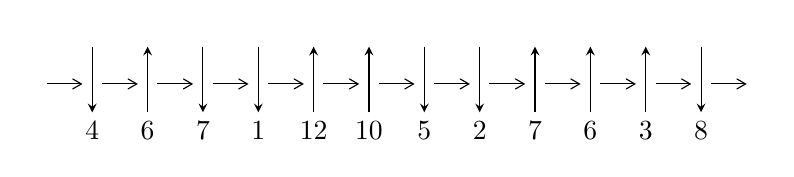
\begin{tikzpicture}[x=20pt, y=17pt]
	% nodes
	\node (C0) at (0, 0) {};
	\node (C1) at (1, 0) {};
	\node (C1U) at (1, +1) {};
	\node (C1D) at (1, -1) {4};

	\node (C2) at (2, 0) {};
	\node (C2U) at (2, +1) {};
	\node (C2D) at (2, -1) {6};

	\node (C3) at (3, 0) {};
	\node (C3U) at (3, +1) {};
	\node (C3D) at (3, -1) {7};

	\node (C4) at (4, 0) {};
	\node (C4U) at (4, +1) {};
	\node (C4D) at (4, -1) {1};

	\node (C5) at (5, 0) {};
	\node (C5U) at (5, +1) {};
	\node (C5D) at (5, -1) {12};

	\node (C6) at (6, 0) {};
	\node (C6U) at (6, +1) {};
	\node (C6D) at (6, -1) {10};

	\node (C7) at (7, 0) {};
	\node (C7U) at (7, +1) {};
	\node (C7D) at (7, -1) {5};

	\node (C8) at (8, 0) {};
	\node (C8U) at (8, +1) {};
	\node (C8D) at (8, -1) {2};

	\node (C9) at (9, 0) {};
	\node (C9U) at (9, +1) {};
	\node (C9D) at (9, -1) {7};

	\node (C10) at (10, 0) {};
	\node (C10U) at (10, +1) {};
	\node (C10D) at (10, -1) {6};

	\node (C11) at (11, 0) {};
	\node (C11U) at (11, +1) {};
	\node (C11D) at (11, -1) {3};

	\node (C12) at (12, 0) {};
	\node (C12U) at (12, +1) {};
	\node (C12D) at (12, -1) {8};
	\node (C13) at (13, 0) {};

	% arrows
	\draw[->,>={angle 60}]
	(C0) edge (C1) (C1) edge (C2) (C2) edge (C3) (C3) edge (C4) (C4) edge (C5) (C5) edge (C6) (C6) edge (C7) (C7) edge (C8) (C8) edge (C9) (C9) edge (C10) (C10) edge (C11) (C11) edge (C12) (C12) edge (C13) ;	\draw[->,>=stealth]
	(C1U) edge (C1D) (C2D) edge (C2U) (C3U) edge (C3D) (C4U) edge (C4D) (C5D) edge (C5U) (C6D) edge (C6U) (C7U) edge (C7D) (C8U) edge (C8D) (C9D) edge (C9U) (C10D) edge (C10U) (C11D) edge (C11U) (C12U) edge (C12D) ;
	\end{tikzpicture} \\
\hhline{~~} \\& 
\textbf{Solving Sequence} \\ \cline{2-2} 
 &
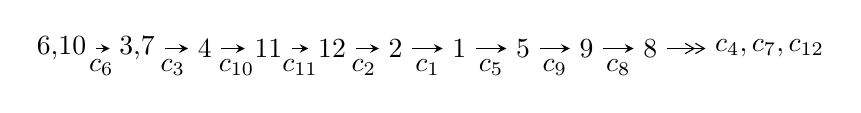
\begin{tikzpicture}[x=23pt, y=7pt]
	% node
	\node (A0) at (-1/8, 0) {6,10};
	\node (A1) at (17/16, 0) {3,7};
	\node (A2) at (17/8, 0) {4};
	\node (A3) at (25/8, 0) {11};
	\node (A4) at (33/8, 0) {12};
	\node (A5) at (41/8, 0) {2};
	\node (A6) at (49/8, 0) {1};
	\node (A7) at (57/8, 0) {5};
	\node (A8) at (65/8, 0) {9};
	\node (A9) at (73/8, 0) {8};
	\node (C1) at (1/2, -1) {$c_{6}$};
	\node (C2) at (13/8, -1) {$c_{3}$};
	\node (C3) at (21/8, -1) {$c_{10}$};
	\node (C4) at (29/8, -1) {$c_{11}$};
	\node (C5) at (37/8, -1) {$c_{2}$};
	\node (C6) at (45/8, -1) {$c_{1}$};
	\node (C7) at (53/8, -1) {$c_{5}$};
	\node (C8) at (61/8, -1) {$c_{9}$};
	\node (C9) at (69/8, -1) {$c_{8}$};
	\node (A10) at (11, 0) {$c_{4},c_{7},c_{12}$};

	% edge
	\draw[->,>=stealth]	
	(A0) edge (A1) (A1) edge (A2) (A2) edge (A3) (A3) edge (A4) (A4) edge (A5) (A5) edge (A6) (A6) edge (A7) (A7) edge (A8) (A8) edge (A9) ;
	\draw[->>,>={angle 60}]	
	(A9) edge (A10);
\end{tikzpicture} \\ 

\end{tabular} \\

\footnotetext{
The image of knot diagram is generated by the software ``\textbf{Draw programme}" developed by Andrew Bartholomew(\url{http://www.layer8.co.uk/maths/draw/index.htm\#Running-draw}), where we modified some parts for our purpose(\url{https://github.com/CATsTAILs/LinksPainter}).
}\phantom \\ \newline 
\centering \textbf{Ideals for irreducible components\footnotemark of $X_{\text{par}}$} 
 
\begin{align*}
I^u_{1}&=\langle 
3.36560\times10^{16} u^{33}-4.05432\times10^{17} u^{32}+\cdots+2.03548\times10^{16} b-4.65631\times10^{16},\\
\phantom{I^u_{1}}&\phantom{= \langle  }4.40305\times10^{16} u^{33}-5.75517\times10^{17} u^{32}+\cdots+4.07095\times10^{16} a-1.59911\times10^{17},\;u^{34}-13 u^{33}+\cdots-6 u+4\rangle \\
I^u_{2}&=\langle 
-164346 u^{11} a^3+243817 u^{11} a^2+\cdots+1429364 a+308156,\;5 u^{11} a^2-2 u^{11} a+\cdots-4 a-3,\\
\phantom{I^u_{2}}&\phantom{= \langle  }u^{12}+5 u^{11}+13 u^{10}+20 u^9+21 u^8+16 u^7+12 u^6+8 u^5+6 u^4+3 u^3+3 u^2+1\rangle \\
I^u_{3}&=\langle 
-127540 u^{19}-1007094 u^{18}+\cdots+123517 b+27064,\\
\phantom{I^u_{3}}&\phantom{= \langle  }-154604 u^{19}-1351146 u^{18}+\cdots+123517 a-395220,\;u^{20}+8 u^{19}+\cdots+u+1\rangle \\
\\
\end{align*}
\raggedright * 3 irreducible components of $\dim_{\mathbb{C}}=0$, with total 102 representations.\\
\footnotetext{All coefficients of polynomials are rational numbers. But the coefficients are sometimes approximated in decimal forms when there is not enough margin.}
\newpage
\renewcommand{\arraystretch}{1}
\centering \section*{I. $I^u_{1}= \langle 3.37\times10^{16} u^{33}-4.05\times10^{17} u^{32}+\cdots+2.04\times10^{16} b-4.66\times10^{16},\;4.40\times10^{16} u^{33}-5.76\times10^{17} u^{32}+\cdots+4.07\times10^{16} a-1.60\times10^{17},\;u^{34}-13 u^{33}+\cdots-6 u+4 \rangle$}
\flushleft \textbf{(i) Arc colorings}\\
\begin{tabular}{m{7pt} m{180pt} m{7pt} m{180pt} }
\flushright $a_{6}=$&$\begin{pmatrix}1\\0\end{pmatrix}$ \\
\flushright $a_{10}=$&$\begin{pmatrix}0\\u\end{pmatrix}$ \\
\flushright $a_{3}=$&$\begin{pmatrix}-1.08158 u^{33}+14.1371 u^{32}+\cdots-1.84914 u+3.92810\\-1.65347 u^{33}+19.9183 u^{32}+\cdots-5.07189 u+2.28758\end{pmatrix}$ \\
\flushright $a_{7}=$&$\begin{pmatrix}1\\- u^2\end{pmatrix}$ \\
\flushright $a_{4}=$&$\begin{pmatrix}-1.00999 u^{33}+11.8197 u^{32}+\cdots-1.56347 u+1.94713\\0.938990 u^{33}-11.3875 u^{32}+\cdots+3.53499 u-3.25944\end{pmatrix}$ \\
\flushright $a_{11}=$&$\begin{pmatrix}u\\u\end{pmatrix}$ \\
\flushright $a_{12}=$&$\begin{pmatrix}0.204732 u^{33}-3.45935 u^{32}+\cdots-6.67202 u+1.64778\\1.28084 u^{33}-16.1679 u^{32}+\cdots+1.50444 u-4.30443\end{pmatrix}$ \\
\flushright $a_{2}=$&$\begin{pmatrix}0.571894 u^{33}-5.78115 u^{32}+\cdots+3.22275 u+1.64052\\-1.65347 u^{33}+19.9183 u^{32}+\cdots-5.07189 u+2.28758\end{pmatrix}$ \\
\flushright $a_{1}=$&$\begin{pmatrix}-0.267000 u^{33}+3.12839 u^{32}+\cdots+0.838672 u+2.49762\\-0.625596 u^{33}+6.10151 u^{32}+\cdots-4.07077 u-2.20949\end{pmatrix}$ \\
\flushright $a_{5}=$&$\begin{pmatrix}4.42916 u^{33}-52.7017 u^{32}+\cdots+19.1323 u-9.10875\\0.312839 u^{33}+0.640403 u^{32}+\cdots+0.133353 u+11.3419\end{pmatrix}$ \\
\flushright $a_{9}=$&$\begin{pmatrix}- u\\u^3+u\end{pmatrix}$ \\
\flushright $a_{8}=$&$\begin{pmatrix}-0.278275 u^{33}+3.49089 u^{32}+\cdots-12.0526 u+6.77114\\0.126689 u^{33}-1.92864 u^{32}+\cdots-4.10149 u-1.11310\end{pmatrix}$\\&\end{tabular}
\flushleft \textbf{(ii) Obstruction class $= -1$}\\~\\
\flushleft \textbf{(iii) Cusp Shapes $= \frac{245172184142911492}{10177386517582189} u^{33}-\frac{2970953353069335864}{10177386517582189} u^{32}+\cdots+\frac{687896807227313368}{10177386517582189} u-\frac{550241350633760298}{10177386517582189}$}\\~\\
\newpage\renewcommand{\arraystretch}{1}
\flushleft \textbf{(iv) u-Polynomials at the component}\newline \\
\begin{tabular}{m{50pt}|m{274pt}}
Crossings & \hspace{64pt}u-Polynomials at each crossing \\
\hline $$\begin{aligned}c_{1},c_{4}\end{aligned}$$&$\begin{aligned}
&u^{34}-15 u^{33}+\cdots-260 u+16
\end{aligned}$\\
\hline $$\begin{aligned}c_{2},c_{11}\end{aligned}$$&$\begin{aligned}
&u^{34}-3 u^{33}+\cdots+u+1
\end{aligned}$\\
\hline $$\begin{aligned}c_{3},c_{8}\end{aligned}$$&$\begin{aligned}
&u^{34}+u^{33}+\cdots+104 u+52
\end{aligned}$\\
\hline $$\begin{aligned}c_{5}\end{aligned}$$&$\begin{aligned}
&u^{34}-24 u^{33}+\cdots-65536 u+4096
\end{aligned}$\\
\hline $$\begin{aligned}c_{6},c_{9},c_{10}\end{aligned}$$&$\begin{aligned}
&u^{34}+13 u^{33}+\cdots+6 u+4
\end{aligned}$\\
\hline $$\begin{aligned}c_{7},c_{12}\end{aligned}$$&$\begin{aligned}
&u^{34}- u^{33}+\cdots+2 u+1
\end{aligned}$\\
\hline
\end{tabular}\\~\\
\newpage\renewcommand{\arraystretch}{1}
\flushleft \textbf{(v) Riley Polynomials at the component}\newline \\
\begin{tabular}{m{50pt}|m{274pt}}
Crossings & \hspace{64pt}Riley Polynomials at each crossing \\
\hline $$\begin{aligned}c_{1},c_{4}\end{aligned}$$&$\begin{aligned}
&y^{34}+25 y^{33}+\cdots+6608 y+256
\end{aligned}$\\
\hline $$\begin{aligned}c_{2},c_{11}\end{aligned}$$&$\begin{aligned}
&y^{34}-37 y^{33}+\cdots-3 y+1
\end{aligned}$\\
\hline $$\begin{aligned}c_{3},c_{8}\end{aligned}$$&$\begin{aligned}
&y^{34}+15 y^{33}+\cdots+26832 y+2704
\end{aligned}$\\
\hline $$\begin{aligned}c_{5}\end{aligned}$$&$\begin{aligned}
&y^{34}+18 y^{33}+\cdots+41943040 y+16777216
\end{aligned}$\\
\hline $$\begin{aligned}c_{6},c_{9},c_{10}\end{aligned}$$&$\begin{aligned}
&y^{34}+13 y^{33}+\cdots+4 y+16
\end{aligned}$\\
\hline $$\begin{aligned}c_{7},c_{12}\end{aligned}$$&$\begin{aligned}
&y^{34}+9 y^{33}+\cdots+24 y+1
\end{aligned}$\\
\hline
\end{tabular}\\~\\
\newpage\flushleft \textbf{(vi) Complex Volumes and Cusp Shapes}
$$\begin{array}{c|c|c}  
\text{Solutions to }I^u_{1}& \I (\text{vol} + \sqrt{-1}CS) & \text{Cusp shape}\\
 \hline 
\begin{aligned}
u &= -0.177745 + 0.860510 I \\
a &= -0.987660 + 0.758962 I \\
b &= -0.133957 + 0.738294 I\end{aligned}
 & -0.48946 - 2.43392 I & -4.03642 + 1.50736 I \\ \hline\begin{aligned}
u &= -0.177745 - 0.860510 I \\
a &= -0.987660 - 0.758962 I \\
b &= -0.133957 - 0.738294 I\end{aligned}
 & -0.48946 + 2.43392 I & -4.03642 - 1.50736 I \\ \hline\begin{aligned}
u &= \phantom{-}0.807369 + 0.789323 I \\
a &= -0.046019 - 1.265130 I \\
b &= -1.54529 - 0.84093 I\end{aligned}
 & \phantom{-}4.30370 + 4.79186 I & \phantom{-}12.7548 - 15.8539 I \\ \hline\begin{aligned}
u &= \phantom{-}0.807369 - 0.789323 I \\
a &= -0.046019 + 1.265130 I \\
b &= -1.54529 + 0.84093 I\end{aligned}
 & \phantom{-}4.30370 - 4.79186 I & \phantom{-}12.7548 + 15.8539 I \\ \hline\begin{aligned}
u &= -0.742638 + 0.428063 I \\
a &= -0.092694 - 1.192120 I \\
b &= -0.201006 - 0.534634 I\end{aligned}
 & \phantom{-}3.50069 - 1.29985 I & \phantom{-}5.39595 + 2.66124 I \\ \hline\begin{aligned}
u &= -0.742638 - 0.428063 I \\
a &= -0.092694 + 1.192120 I \\
b &= -0.201006 + 0.534634 I\end{aligned}
 & \phantom{-}3.50069 + 1.29985 I & \phantom{-}5.39595 - 2.66124 I \\ \hline\begin{aligned}
u &= -0.199740 + 0.757222 I \\
a &= \phantom{-}0.768202 + 1.019930 I \\
b &= \phantom{-}0.694012 + 0.122979 I\end{aligned}
 & \phantom{-}1.79897 - 2.51887 I & \phantom{-}1.62969 + 2.73665 I \\ \hline\begin{aligned}
u &= -0.199740 - 0.757222 I \\
a &= \phantom{-}0.768202 - 1.019930 I \\
b &= \phantom{-}0.694012 - 0.122979 I\end{aligned}
 & \phantom{-}1.79897 + 2.51887 I & \phantom{-}1.62969 - 2.73665 I \\ \hline\begin{aligned}
u &= \phantom{-}0.807251 + 0.921530 I \\
a &= -0.549456 - 1.161350 I \\
b &= -1.63739 - 0.33756 I\end{aligned}
 & \phantom{-}4.49772 + 3.04334 I & \phantom{-0.000000 } 0 \\ \hline\begin{aligned}
u &= \phantom{-}0.807251 - 0.921530 I \\
a &= -0.549456 + 1.161350 I \\
b &= -1.63739 + 0.33756 I\end{aligned}
 & \phantom{-}4.49772 - 3.04334 I & \phantom{-0.000000 } 0\\
 \hline 
 \end{array}$$\newpage$$\begin{array}{c|c|c}  
\text{Solutions to }I^u_{1}& \I (\text{vol} + \sqrt{-1}CS) & \text{Cusp shape}\\
 \hline 
\begin{aligned}
u &= \phantom{-}0.968837 + 0.772002 I \\
a &= \phantom{-}0.600368 + 0.589855 I \\
b &= \phantom{-}1.331840 - 0.217349 I\end{aligned}
 & \phantom{-}1.19675 - 4.92326 I & \phantom{-0.000000 } 0 \\ \hline\begin{aligned}
u &= \phantom{-}0.968837 - 0.772002 I \\
a &= \phantom{-}0.600368 - 0.589855 I \\
b &= \phantom{-}1.331840 + 0.217349 I\end{aligned}
 & \phantom{-}1.19675 + 4.92326 I & \phantom{-0.000000 } 0 \\ \hline\begin{aligned}
u &= \phantom{-}0.704114 + 1.059300 I \\
a &= -0.900068 - 0.778966 I \\
b &= -1.362050 + 0.199758 I\end{aligned}
 & \phantom{-}3.45060 + 0.99312 I & \phantom{-0.000000 } 0 \\ \hline\begin{aligned}
u &= \phantom{-}0.704114 - 1.059300 I \\
a &= -0.900068 + 0.778966 I \\
b &= -1.362050 - 0.199758 I\end{aligned}
 & \phantom{-}3.45060 - 0.99312 I & \phantom{-0.000000 } 0 \\ \hline\begin{aligned}
u &= \phantom{-}1.086830 + 0.767498 I \\
a &= \phantom{-}0.484855 + 0.792427 I \\
b &= \phantom{-}1.57485 + 0.28400 I\end{aligned}
 & \phantom{-}10.11120 - 2.61148 I & \phantom{-0.000000 } 0 \\ \hline\begin{aligned}
u &= \phantom{-}1.086830 - 0.767498 I \\
a &= \phantom{-}0.484855 - 0.792427 I \\
b &= \phantom{-}1.57485 - 0.28400 I\end{aligned}
 & \phantom{-}10.11120 + 2.61148 I & \phantom{-0.000000 } 0 \\ \hline\begin{aligned}
u &= \phantom{-}0.878326 + 1.055870 I \\
a &= \phantom{-}0.371450 + 1.291500 I \\
b &= \phantom{-}1.53857 + 0.80521 I\end{aligned}
 & \phantom{-}0.37459 + 11.68900 I & \phantom{-0.000000 } 0 \\ \hline\begin{aligned}
u &= \phantom{-}0.878326 - 1.055870 I \\
a &= \phantom{-}0.371450 - 1.291500 I \\
b &= \phantom{-}1.53857 - 0.80521 I\end{aligned}
 & \phantom{-}0.37459 - 11.68900 I & \phantom{-0.000000 } 0 \\ \hline\begin{aligned}
u &= -0.386020 + 0.458150 I \\
a &= -0.537326 + 0.629358 I \\
b &= -0.052527 + 0.335533 I\end{aligned}
 & \phantom{-}0.064441 - 1.136870 I & \phantom{-}0.93772 + 5.85683 I \\ \hline\begin{aligned}
u &= -0.386020 - 0.458150 I \\
a &= -0.537326 - 0.629358 I \\
b &= -0.052527 - 0.335533 I\end{aligned}
 & \phantom{-}0.064441 + 1.136870 I & \phantom{-}0.93772 - 5.85683 I\\
 \hline 
 \end{array}$$\newpage$$\begin{array}{c|c|c}  
\text{Solutions to }I^u_{1}& \I (\text{vol} + \sqrt{-1}CS) & \text{Cusp shape}\\
 \hline 
\begin{aligned}
u &= \phantom{-}0.89212 + 1.15663 I \\
a &= \phantom{-}0.747140 + 1.031830 I \\
b &= \phantom{-}1.57182 + 0.30895 I\end{aligned}
 & \phantom{-}8.86289 + 9.81740 I & \phantom{-0.000000 } 0 \\ \hline\begin{aligned}
u &= \phantom{-}0.89212 - 1.15663 I \\
a &= \phantom{-}0.747140 - 1.031830 I \\
b &= \phantom{-}1.57182 - 0.30895 I\end{aligned}
 & \phantom{-}8.86289 - 9.81740 I & \phantom{-0.000000 } 0 \\ \hline\begin{aligned}
u &= \phantom{-}1.22079 + 0.87455 I \\
a &= -0.716079 - 0.451230 I \\
b &= -1.395450 + 0.196055 I\end{aligned}
 & \phantom{-}6.07747 - 9.60440 I & \phantom{-0.000000 } 0 \\ \hline\begin{aligned}
u &= \phantom{-}1.22079 - 0.87455 I \\
a &= -0.716079 + 0.451230 I \\
b &= -1.395450 - 0.196055 I\end{aligned}
 & \phantom{-}6.07747 + 9.60440 I & \phantom{-0.000000 } 0 \\ \hline\begin{aligned}
u &= \phantom{-}0.98696 + 1.14798 I \\
a &= -0.477391 - 1.245850 I \\
b &= -1.55779 - 0.81772 I\end{aligned}
 & \phantom{-}5.1283 + 17.4721 I & \phantom{-0.000000 } 0 \\ \hline\begin{aligned}
u &= \phantom{-}0.98696 - 1.14798 I \\
a &= -0.477391 + 1.245850 I \\
b &= -1.55779 + 0.81772 I\end{aligned}
 & \phantom{-}5.1283 - 17.4721 I & \phantom{-0.000000 } 0 \\ \hline\begin{aligned}
u &= -0.00685 + 1.55539 I \\
a &= \phantom{-}0.394264 + 0.143907 I \\
b &= \phantom{-}0.343831 - 0.076929 I\end{aligned}
 & -7.56742 - 2.39125 I & \phantom{-0.000000 } 0 \\ \hline\begin{aligned}
u &= -0.00685 - 1.55539 I \\
a &= \phantom{-}0.394264 - 0.143907 I \\
b &= \phantom{-}0.343831 + 0.076929 I\end{aligned}
 & -7.56742 + 2.39125 I & \phantom{-0.000000 } 0 \\ \hline\begin{aligned}
u &= \phantom{-}0.201303 + 0.350187 I \\
a &= \phantom{-}1.40378 - 2.09303 I \\
b &= -1.034130 - 0.541372 I\end{aligned}
 & \phantom{-}1.50426 + 2.26332 I & \phantom{-}0.52367 - 3.19533 I \\ \hline\begin{aligned}
u &= \phantom{-}0.201303 - 0.350187 I \\
a &= \phantom{-}1.40378 + 2.09303 I \\
b &= -1.034130 + 0.541372 I\end{aligned}
 & \phantom{-}1.50426 - 2.26332 I & \phantom{-}0.52367 + 3.19533 I\\
 \hline 
 \end{array}$$\newpage$$\begin{array}{c|c|c}  
\text{Solutions to }I^u_{1}& \I (\text{vol} + \sqrt{-1}CS) & \text{Cusp shape}\\
 \hline 
\begin{aligned}
u &= -0.399608 + 0.017982 I \\
a &= \phantom{-}2.46321 - 2.18711 I \\
b &= \phantom{-}0.683499 - 0.647318 I\end{aligned}
 & \phantom{-}1.77799 - 2.09204 I & -0.21369 + 3.52332 I \\ \hline\begin{aligned}
u &= -0.399608 - 0.017982 I \\
a &= \phantom{-}2.46321 + 2.18711 I \\
b &= \phantom{-}0.683499 + 0.647318 I\end{aligned}
 & \phantom{-}1.77799 + 2.09204 I & -0.21369 - 3.52332 I \\ \hline\begin{aligned}
u &= -0.14129 + 1.69680 I \\
a &= -0.176576 - 0.469335 I \\
b &= -0.318827 - 0.269592 I\end{aligned}
 & -5.11425 - 5.43935 I & \phantom{-0.000000 } 0 \\ \hline\begin{aligned}
u &= -0.14129 - 1.69680 I \\
a &= -0.176576 + 0.469335 I \\
b &= -0.318827 + 0.269592 I\end{aligned}
 & -5.11425 + 5.43935 I & \phantom{-0.000000 } 0\\
 \hline 
 \end{array}$$\newpage\newpage\renewcommand{\arraystretch}{1}
\centering \section*{II. $I^u_{2}= \langle -1.64\times10^{5} a^{3} u^{11}+2.44\times10^{5} a^{2} u^{11}+\cdots+1.43\times10^{6} a+3.08\times10^{5},\;5 u^{11} a^2-2 u^{11} a+\cdots-4 a-3,\;u^{12}+5 u^{11}+\cdots+3 u^2+1 \rangle$}
\flushleft \textbf{(i) Arc colorings}\\
\begin{tabular}{m{7pt} m{180pt} m{7pt} m{180pt} }
\flushright $a_{6}=$&$\begin{pmatrix}1\\0\end{pmatrix}$ \\
\flushright $a_{10}=$&$\begin{pmatrix}0\\u\end{pmatrix}$ \\
\flushright $a_{3}=$&$\begin{pmatrix}a\\0.173165 a^{3} u^{11}-0.256901 a^{2} u^{11}+\cdots-1.50607 a-0.324693\end{pmatrix}$ \\
\flushright $a_{7}=$&$\begin{pmatrix}1\\- u^2\end{pmatrix}$ \\
\flushright $a_{4}=$&$\begin{pmatrix}-0.173165 a^{3} u^{11}+0.256901 a^{2} u^{11}+\cdots+2.50607 a+0.324693\\0.0438292 a^{3} u^{11}+0.198053 a^{2} u^{11}+\cdots-0.0752979 a+0.187445\end{pmatrix}$ \\
\flushright $a_{11}=$&$\begin{pmatrix}u\\u\end{pmatrix}$ \\
\flushright $a_{12}=$&$\begin{pmatrix}0.233575 a^{3} u^{11}-0.244925 a^{2} u^{11}+\cdots-0.00431686 a-0.0487698\\-0.137377 a^{3} u^{11}-0.991313 a^{2} u^{11}+\cdots-0.124280 a+0.0462769\end{pmatrix}$ \\
\flushright $a_{2}=$&$\begin{pmatrix}-0.173165 a^{3} u^{11}+0.256901 a^{2} u^{11}+\cdots+2.50607 a+0.324693\\0.173165 a^{3} u^{11}-0.256901 a^{2} u^{11}+\cdots-1.50607 a-0.324693\end{pmatrix}$ \\
\flushright $a_{1}=$&$\begin{pmatrix}-0.590217 a^{3} u^{11}-0.580359 a^{2} u^{11}+\cdots+2.60386 a+1.74028\\0.384443 a^{3} u^{11}+0.245718 a^{2} u^{11}+\cdots-0.729774 a-1.29352\end{pmatrix}$ \\
\flushright $a_{5}=$&$\begin{pmatrix}0.482755 a^{3} u^{11}+0.427855 a^{2} u^{11}+\cdots+0.290788 a+1.76402\\-0.137377 a^{3} u^{11}-0.991313 a^{2} u^{11}+\cdots-0.124280 a-0.953723\end{pmatrix}$ \\
\flushright $a_{9}=$&$\begin{pmatrix}- u\\u^3+u\end{pmatrix}$ \\
\flushright $a_{8}=$&$\begin{pmatrix}-0.808272 a^{3} u^{11}-0.111891 a^{2} u^{11}+\cdots+0.482231 a+0.268134\\1.17922 a^{3} u^{11}+0.858278 a^{2} u^{11}+\cdots-0.362268 a-0.363181\end{pmatrix}$\\&\end{tabular}
\flushleft \textbf{(ii) Obstruction class $= -1$}\\~\\
\flushleft \textbf{(iii) Cusp Shapes $= \frac{52152}{94907} u^{11} a^3+\frac{376330}{94907} u^{11} a^2+\cdots+\frac{47180}{94907} a-\frac{1346266}{94907}$}\\~\\
\newpage\renewcommand{\arraystretch}{1}
\flushleft \textbf{(iv) u-Polynomials at the component}\newline \\
\begin{tabular}{m{50pt}|m{274pt}}
Crossings & \hspace{64pt}u-Polynomials at each crossing \\
\hline $$\begin{aligned}c_{1},c_{4}\end{aligned}$$&$\begin{aligned}
&(u^{12}+3 u^{11}+\cdots-2 u+1)^{4}
\end{aligned}$\\
\hline $$\begin{aligned}c_{2},c_{11}\end{aligned}$$&$\begin{aligned}
&u^{48}-3 u^{47}+\cdots-1764 u+304
\end{aligned}$\\
\hline $$\begin{aligned}c_{3},c_{8}\end{aligned}$$&$\begin{aligned}
&u^{48}- u^{47}+\cdots-10752 u+31744
\end{aligned}$\\
\hline $$\begin{aligned}c_{5}\end{aligned}$$&$\begin{aligned}
&(u^2+u+1)^{24}
\end{aligned}$\\
\hline $$\begin{aligned}c_{6},c_{9},c_{10}\end{aligned}$$&$\begin{aligned}
&(u^{12}-5 u^{11}+\cdots+3 u^2+1)^{4}
\end{aligned}$\\
\hline $$\begin{aligned}c_{7},c_{12}\end{aligned}$$&$\begin{aligned}
&u^{48}+u^{47}+\cdots-8 u+4
\end{aligned}$\\
\hline
\end{tabular}\\~\\
\newpage\renewcommand{\arraystretch}{1}
\flushleft \textbf{(v) Riley Polynomials at the component}\newline \\
\begin{tabular}{m{50pt}|m{274pt}}
Crossings & \hspace{64pt}Riley Polynomials at each crossing \\
\hline $$\begin{aligned}c_{1},c_{4}\end{aligned}$$&$\begin{aligned}
&(y^{12}+9 y^{11}+\cdots-6 y+1)^{4}
\end{aligned}$\\
\hline $$\begin{aligned}c_{2},c_{11}\end{aligned}$$&$\begin{aligned}
&y^{48}-25 y^{47}+\cdots-3021104 y+92416
\end{aligned}$\\
\hline $$\begin{aligned}c_{3},c_{8}\end{aligned}$$&$\begin{aligned}
&y^{48}+19 y^{47}+\cdots-4422631424 y+1007681536
\end{aligned}$\\
\hline $$\begin{aligned}c_{5}\end{aligned}$$&$\begin{aligned}
&(y^2+y+1)^{24}
\end{aligned}$\\
\hline $$\begin{aligned}c_{6},c_{9},c_{10}\end{aligned}$$&$\begin{aligned}
&(y^{12}+y^{11}+\cdots+6 y+1)^{4}
\end{aligned}$\\
\hline $$\begin{aligned}c_{7},c_{12}\end{aligned}$$&$\begin{aligned}
&y^{48}-9 y^{47}+\cdots+648 y+16
\end{aligned}$\\
\hline
\end{tabular}\\~\\
\newpage\flushleft \textbf{(vi) Complex Volumes and Cusp Shapes}
$$\begin{array}{c|c|c}  
\text{Solutions to }I^u_{2}& \I (\text{vol} + \sqrt{-1}CS) & \text{Cusp shape}\\
 \hline 
\begin{aligned}
u &= -0.096849 + 0.815314 I \\
a &= -0.991274 + 0.244561 I \\
b &= \phantom{-}0.180533 + 0.571823 I\end{aligned}
 & -0.55801 - 2.43094 I & -5.64801 + 1.26417 I \\ \hline\begin{aligned}
u &= -0.096849 + 0.815314 I \\
a &= -0.334752 + 0.461645 I \\
b &= -1.62106 + 0.09220 I\end{aligned}
 & -0.55801 - 6.49071 I & -5.64801 + 8.19237 I \\ \hline\begin{aligned}
u &= -0.096849 + 0.815314 I \\
a &= -1.04597 + 1.22420 I \\
b &= -0.380309 + 0.923695 I\end{aligned}
 & -0.55801 - 2.43094 I & -5.64801 + 1.26417 I \\ \hline\begin{aligned}
u &= -0.096849 + 0.815314 I \\
a &= \phantom{-}0.08139 - 2.96033 I \\
b &= \phantom{-}0.425795 - 1.012970 I\end{aligned}
 & -0.55801 - 6.49071 I & -5.64801 + 8.19237 I \\ \hline\begin{aligned}
u &= -0.096849 - 0.815314 I \\
a &= -0.991274 - 0.244561 I \\
b &= \phantom{-}0.180533 - 0.571823 I\end{aligned}
 & -0.55801 + 2.43094 I & -5.64801 - 1.26417 I \\ \hline\begin{aligned}
u &= -0.096849 - 0.815314 I \\
a &= -0.334752 - 0.461645 I \\
b &= -1.62106 - 0.09220 I\end{aligned}
 & -0.55801 + 6.49071 I & -5.64801 - 8.19237 I \\ \hline\begin{aligned}
u &= -0.096849 - 0.815314 I \\
a &= -1.04597 - 1.22420 I \\
b &= -0.380309 - 0.923695 I\end{aligned}
 & -0.55801 + 2.43094 I & -5.64801 - 1.26417 I \\ \hline\begin{aligned}
u &= -0.096849 - 0.815314 I \\
a &= \phantom{-}0.08139 + 2.96033 I \\
b &= \phantom{-}0.425795 + 1.012970 I\end{aligned}
 & -0.55801 + 6.49071 I & -5.64801 - 8.19237 I \\ \hline\begin{aligned}
u &= -0.897414 + 0.962359 I \\
a &= -0.512515 + 0.835613 I \\
b &= -1.54234 + 0.56752 I\end{aligned}
 & \phantom{-}1.93740 - 5.36645 I & -3.82297 + 5.38834 I \\ \hline\begin{aligned}
u &= -0.897414 + 0.962359 I \\
a &= -0.635177 + 0.979032 I \\
b &= -1.154690 + 0.241144 I\end{aligned}
 & \phantom{-}1.93740 - 1.30669 I & -3.82297 - 1.53987 I\\
 \hline 
 \end{array}$$\newpage$$\begin{array}{c|c|c}  
\text{Solutions to }I^u_{2}& \I (\text{vol} + \sqrt{-1}CS) & \text{Cusp shape}\\
 \hline 
\begin{aligned}
u &= -0.897414 + 0.962359 I \\
a &= \phantom{-}0.067373 - 1.313560 I \\
b &= \phantom{-}1.182180 - 0.750468 I\end{aligned}
 & \phantom{-}1.93740 - 5.36645 I & -3.82297 + 5.38834 I \\ \hline\begin{aligned}
u &= -0.897414 + 0.962359 I \\
a &= \phantom{-}0.443837 - 0.354556 I \\
b &= \phantom{-}1.176330 + 0.162236 I\end{aligned}
 & \phantom{-}1.93740 - 1.30669 I & -3.82297 - 1.53987 I \\ \hline\begin{aligned}
u &= -0.897414 - 0.962359 I \\
a &= -0.512515 - 0.835613 I \\
b &= -1.54234 - 0.56752 I\end{aligned}
 & \phantom{-}1.93740 + 5.36645 I & -3.82297 - 5.38834 I \\ \hline\begin{aligned}
u &= -0.897414 - 0.962359 I \\
a &= -0.635177 - 0.979032 I \\
b &= -1.154690 - 0.241144 I\end{aligned}
 & \phantom{-}1.93740 + 1.30669 I & -3.82297 + 1.53987 I \\ \hline\begin{aligned}
u &= -0.897414 - 0.962359 I \\
a &= \phantom{-}0.067373 + 1.313560 I \\
b &= \phantom{-}1.182180 + 0.750468 I\end{aligned}
 & \phantom{-}1.93740 + 5.36645 I & -3.82297 - 5.38834 I \\ \hline\begin{aligned}
u &= -0.897414 - 0.962359 I \\
a &= \phantom{-}0.443837 + 0.354556 I \\
b &= \phantom{-}1.176330 - 0.162236 I\end{aligned}
 & \phantom{-}1.93740 + 1.30669 I & -3.82297 + 1.53987 I \\ \hline\begin{aligned}
u &= \phantom{-}0.492148 + 0.450600 I \\
a &= \phantom{-}1.238170 + 0.532971 I \\
b &= -0.806292 - 0.362544 I\end{aligned}
 & \phantom{-}1.25303 + 4.19921 I & \phantom{-}2.04009 - 7.81755 I \\ \hline\begin{aligned}
u &= \phantom{-}0.492148 + 0.450600 I \\
a &= -0.45433 + 1.76693 I \\
b &= -0.60135 + 2.02277 I\end{aligned}
 & \phantom{-}1.25303 + 8.25898 I & \phantom{-}2.0401 - 14.7458 I \\ \hline\begin{aligned}
u &= \phantom{-}0.492148 + 0.450600 I \\
a &= \phantom{-}0.65546 - 1.77721 I \\
b &= -0.60266 - 1.36196 I\end{aligned}
 & \phantom{-}1.25303 + 4.19921 I & \phantom{-}2.04009 - 7.81755 I \\ \hline\begin{aligned}
u &= \phantom{-}0.492148 + 0.450600 I \\
a &= -1.57002 - 2.78474 I \\
b &= -0.187637 + 0.059665 I\end{aligned}
 & \phantom{-}1.25303 + 8.25898 I & \phantom{-}2.0401 - 14.7458 I\\
 \hline 
 \end{array}$$\newpage$$\begin{array}{c|c|c}  
\text{Solutions to }I^u_{2}& \I (\text{vol} + \sqrt{-1}CS) & \text{Cusp shape}\\
 \hline 
\begin{aligned}
u &= \phantom{-}0.492148 - 0.450600 I \\
a &= \phantom{-}1.238170 - 0.532971 I \\
b &= -0.806292 + 0.362544 I\end{aligned}
 & \phantom{-}1.25303 - 4.19921 I & \phantom{-}2.04009 + 7.81755 I \\ \hline\begin{aligned}
u &= \phantom{-}0.492148 - 0.450600 I \\
a &= -0.45433 - 1.76693 I \\
b &= -0.60135 - 2.02277 I\end{aligned}
 & \phantom{-}1.25303 - 8.25898 I & \phantom{-}2.0401 + 14.7458 I \\ \hline\begin{aligned}
u &= \phantom{-}0.492148 - 0.450600 I \\
a &= \phantom{-}0.65546 + 1.77721 I \\
b &= -0.60266 + 1.36196 I\end{aligned}
 & \phantom{-}1.25303 - 4.19921 I & \phantom{-}2.04009 + 7.81755 I \\ \hline\begin{aligned}
u &= \phantom{-}0.492148 - 0.450600 I \\
a &= -1.57002 + 2.78474 I \\
b &= -0.187637 - 0.059665 I\end{aligned}
 & \phantom{-}1.25303 - 8.25898 I & \phantom{-}2.0401 + 14.7458 I \\ \hline\begin{aligned}
u &= \phantom{-}0.225615 + 0.583583 I \\
a &= \phantom{-}0.49226 - 1.52837 I \\
b &= \phantom{-}0.30789 - 1.81604 I\end{aligned}
 & -3.58098 + 2.94957 I & -9.5307 - 10.6461 I \\ \hline\begin{aligned}
u &= \phantom{-}0.225615 + 0.583583 I \\
a &= -0.0844684 - 0.0883145 I \\
b &= \phantom{-}1.43468 + 0.37842 I\end{aligned}
 & -3.58098 - 1.11020 I & -9.53074 - 3.71786 I \\ \hline\begin{aligned}
u &= \phantom{-}0.225615 + 0.583583 I \\
a &= \phantom{-}2.65608 + 1.33311 I \\
b &= \phantom{-}0.126282 - 0.172499 I\end{aligned}
 & -3.58098 + 2.94957 I & -9.5307 - 10.6461 I \\ \hline\begin{aligned}
u &= \phantom{-}0.225615 + 0.583583 I \\
a &= -1.32060 + 2.91249 I \\
b &= \phantom{-}0.070364 + 0.991849 I\end{aligned}
 & -3.58098 - 1.11020 I & -9.53074 - 3.71786 I \\ \hline\begin{aligned}
u &= \phantom{-}0.225615 - 0.583583 I \\
a &= \phantom{-}0.49226 + 1.52837 I \\
b &= \phantom{-}0.30789 + 1.81604 I\end{aligned}
 & -3.58098 - 2.94957 I & -9.5307 + 10.6461 I \\ \hline\begin{aligned}
u &= \phantom{-}0.225615 - 0.583583 I \\
a &= -0.0844684 + 0.0883145 I \\
b &= \phantom{-}1.43468 - 0.37842 I\end{aligned}
 & -3.58098 + 1.11020 I & -9.53074 + 3.71786 I\\
 \hline 
 \end{array}$$\newpage$$\begin{array}{c|c|c}  
\text{Solutions to }I^u_{2}& \I (\text{vol} + \sqrt{-1}CS) & \text{Cusp shape}\\
 \hline 
\begin{aligned}
u &= \phantom{-}0.225615 - 0.583583 I \\
a &= \phantom{-}2.65608 - 1.33311 I \\
b &= \phantom{-}0.126282 + 0.172499 I\end{aligned}
 & -3.58098 - 2.94957 I & -9.5307 + 10.6461 I \\ \hline\begin{aligned}
u &= \phantom{-}0.225615 - 0.583583 I \\
a &= -1.32060 - 2.91249 I \\
b &= \phantom{-}0.070364 - 0.991849 I\end{aligned}
 & -3.58098 + 1.11020 I & -9.53074 + 3.71786 I \\ \hline\begin{aligned}
u &= -1.216860 + 0.709160 I \\
a &= -0.953155 + 0.065735 I \\
b &= -1.62157 - 0.26350 I\end{aligned}
 & \phantom{-}6.16619 - 0.50759 I & \phantom{-}8.43865 - 1.75135 I \\ \hline\begin{aligned}
u &= -1.216860 + 0.709160 I \\
a &= \phantom{-}0.146312 - 0.814725 I \\
b &= \phantom{-}1.046850 - 0.073374 I\end{aligned}
 & \phantom{-}6.16619 - 0.50759 I & \phantom{-}8.43865 - 1.75135 I \\ \hline\begin{aligned}
u &= -1.216860 + 0.709160 I \\
a &= \phantom{-}0.881067 - 0.903352 I \\
b &= \phantom{-}1.74042 - 0.74034 I\end{aligned}
 & \phantom{-}6.16619 - 4.56735 I & \phantom{-}8.43865 + 5.17685 I \\ \hline\begin{aligned}
u &= -1.216860 + 0.709160 I \\
a &= \phantom{-}0.171000 + 0.579101 I \\
b &= -1.161320 + 0.411057 I\end{aligned}
 & \phantom{-}6.16619 - 4.56735 I & \phantom{-}8.43865 + 5.17685 I \\ \hline\begin{aligned}
u &= -1.216860 - 0.709160 I \\
a &= -0.953155 - 0.065735 I \\
b &= -1.62157 + 0.26350 I\end{aligned}
 & \phantom{-}6.16619 + 0.50759 I & \phantom{-}8.43865 + 1.75135 I \\ \hline\begin{aligned}
u &= -1.216860 - 0.709160 I \\
a &= \phantom{-}0.146312 + 0.814725 I \\
b &= \phantom{-}1.046850 + 0.073374 I\end{aligned}
 & \phantom{-}6.16619 + 0.50759 I & \phantom{-}8.43865 + 1.75135 I \\ \hline\begin{aligned}
u &= -1.216860 - 0.709160 I \\
a &= \phantom{-}0.881067 + 0.903352 I \\
b &= \phantom{-}1.74042 + 0.74034 I\end{aligned}
 & \phantom{-}6.16619 + 4.56735 I & \phantom{-}8.43865 - 5.17685 I \\ \hline\begin{aligned}
u &= -1.216860 - 0.709160 I \\
a &= \phantom{-}0.171000 - 0.579101 I \\
b &= -1.161320 - 0.411057 I\end{aligned}
 & \phantom{-}6.16619 + 4.56735 I & \phantom{-}8.43865 - 5.17685 I\\
 \hline 
 \end{array}$$\newpage$$\begin{array}{c|c|c}  
\text{Solutions to }I^u_{2}& \I (\text{vol} + \sqrt{-1}CS) & \text{Cusp shape}\\
 \hline 
\begin{aligned}
u &= -1.00664 + 1.21018 I \\
a &= \phantom{-}0.368637 - 0.732620 I \\
b &= \phantom{-}1.42346 - 0.46423 I\end{aligned}
 & \phantom{-}4.65197 - 7.43387 I & \phantom{-}4.52298 + 12.02747 I \\ \hline\begin{aligned}
u &= -1.00664 + 1.21018 I \\
a &= \phantom{-}1.052560 - 0.811213 I \\
b &= \phantom{-}1.47525 - 0.31651 I\end{aligned}
 & \phantom{-}4.65197 - 3.37411 I & \phantom{-}4.52298 + 5.09926 I \\ \hline\begin{aligned}
u &= -1.00664 + 1.21018 I \\
a &= -0.270267 + 0.605480 I \\
b &= -1.024180 + 0.013550 I\end{aligned}
 & \phantom{-}4.65197 - 3.37411 I & \phantom{-}4.52298 + 5.09926 I \\ \hline\begin{aligned}
u &= -1.00664 + 1.21018 I \\
a &= -0.58161 + 1.51297 I \\
b &= -1.38663 + 1.00635 I\end{aligned}
 & \phantom{-}4.65197 - 7.43387 I & \phantom{-}4.52298 + 12.02747 I \\ \hline\begin{aligned}
u &= -1.00664 - 1.21018 I \\
a &= \phantom{-}0.368637 + 0.732620 I \\
b &= \phantom{-}1.42346 + 0.46423 I\end{aligned}
 & \phantom{-}4.65197 + 7.43387 I & \phantom{-}4.52298 - 12.02747 I \\ \hline\begin{aligned}
u &= -1.00664 - 1.21018 I \\
a &= \phantom{-}1.052560 + 0.811213 I \\
b &= \phantom{-}1.47525 + 0.31651 I\end{aligned}
 & \phantom{-}4.65197 + 3.37411 I & \phantom{-}4.52298 - 5.09926 I \\ \hline\begin{aligned}
u &= -1.00664 - 1.21018 I \\
a &= -0.270267 - 0.605480 I \\
b &= -1.024180 - 0.013550 I\end{aligned}
 & \phantom{-}4.65197 + 3.37411 I & \phantom{-}4.52298 - 5.09926 I \\ \hline\begin{aligned}
u &= -1.00664 - 1.21018 I \\
a &= -0.58161 - 1.51297 I \\
b &= -1.38663 - 1.00635 I\end{aligned}
 & \phantom{-}4.65197 + 7.43387 I & \phantom{-}4.52298 - 12.02747 I\\
 \hline 
 \end{array}$$\newpage\newpage\renewcommand{\arraystretch}{1}
\centering \section*{III. $I^u_{3}= \langle -1.28\times10^{5} u^{19}-1.01\times10^{6} u^{18}+\cdots+1.24\times10^{5} b+2.71\times10^{4},\;-1.55\times10^{5} u^{19}-1.35\times10^{6} u^{18}+\cdots+1.24\times10^{5} a-3.95\times10^{5},\;u^{20}+8 u^{19}+\cdots+u+1 \rangle$}
\flushleft \textbf{(i) Arc colorings}\\
\begin{tabular}{m{7pt} m{180pt} m{7pt} m{180pt} }
\flushright $a_{6}=$&$\begin{pmatrix}1\\0\end{pmatrix}$ \\
\flushright $a_{10}=$&$\begin{pmatrix}0\\u\end{pmatrix}$ \\
\flushright $a_{3}=$&$\begin{pmatrix}1.25168 u^{19}+10.9389 u^{18}+\cdots+5.92810 u+3.19972\\1.03257 u^{19}+8.15348 u^{18}+\cdots+3.19972 u-0.219112\end{pmatrix}$ \\
\flushright $a_{7}=$&$\begin{pmatrix}1\\- u^2\end{pmatrix}$ \\
\flushright $a_{4}=$&$\begin{pmatrix}0.685072 u^{19}+6.77196 u^{18}+\cdots+4.90555 u+4.34433\\0.994365 u^{19}+7.79298 u^{18}+\cdots+2.99900 u+0.146781\end{pmatrix}$ \\
\flushright $a_{11}=$&$\begin{pmatrix}u\\u\end{pmatrix}$ \\
\flushright $a_{12}=$&$\begin{pmatrix}1.41270 u^{19}+10.8173 u^{18}+\cdots+2.62466 u-3.71599\\-0.0514585 u^{19}-0.844532 u^{18}+\cdots-2.71599 u-1.46416\end{pmatrix}$ \\
\flushright $a_{2}=$&$\begin{pmatrix}0.219112 u^{19}+2.78546 u^{18}+\cdots+2.72838 u+3.41883\\1.03257 u^{19}+8.15348 u^{18}+\cdots+3.19972 u-0.219112\end{pmatrix}$ \\
\flushright $a_{1}=$&$\begin{pmatrix}-0.372111 u^{19}-3.33171 u^{18}+\cdots-5.09162 u-1.99085\\0.0253083 u^{19}+0.0849600 u^{18}+\cdots-0.193803 u-0.124768\end{pmatrix}$ \\
\flushright $a_{5}=$&$\begin{pmatrix}-0.0850814 u^{19}-0.341281 u^{18}+\cdots+7.95479 u+5.36282\\0.182671 u^{19}+1.18521 u^{18}+\cdots+2.89866 u+0.319211\end{pmatrix}$ \\
\flushright $a_{9}=$&$\begin{pmatrix}- u\\u^3+u\end{pmatrix}$ \\
\flushright $a_{8}=$&$\begin{pmatrix}0.979841 u^{19}+7.65593 u^{18}+\cdots-0.788045 u-3.66453\\-0.182793 u^{19}-1.80174 u^{18}+\cdots-3.64437 u-0.979841\end{pmatrix}$\\&\end{tabular}
\flushleft \textbf{(ii) Obstruction class $= 1$}\\~\\
\flushleft \textbf{(iii) Cusp Shapes $= -\frac{499031}{123517} u^{19}-\frac{4050048}{123517} u^{18}+\cdots-\frac{2050088}{123517} u-\frac{1463308}{123517}$}\\~\\
\newpage\renewcommand{\arraystretch}{1}
\flushleft \textbf{(iv) u-Polynomials at the component}\newline \\
\begin{tabular}{m{50pt}|m{274pt}}
Crossings & \hspace{64pt}u-Polynomials at each crossing \\
\hline $$\begin{aligned}c_{1}\end{aligned}$$&$\begin{aligned}
&u^{20}-6 u^{19}+\cdots-60 u+13
\end{aligned}$\\
\hline $$\begin{aligned}c_{2},c_{11}\end{aligned}$$&$\begin{aligned}
&u^{20}+u^{19}+\cdots-2 u+1
\end{aligned}$\\
\hline $$\begin{aligned}c_{3},c_{8}\end{aligned}$$&$\begin{aligned}
&u^{20}+u^{19}+\cdots+14 u+4
\end{aligned}$\\
\hline $$\begin{aligned}c_{4}\end{aligned}$$&$\begin{aligned}
&u^{20}+6 u^{19}+\cdots+60 u+13
\end{aligned}$\\
\hline $$\begin{aligned}c_{5}\end{aligned}$$&$\begin{aligned}
&u^{20}+u^{19}+\cdots+16 u+4
\end{aligned}$\\
\hline $$\begin{aligned}c_{6}\end{aligned}$$&$\begin{aligned}
&u^{20}+8 u^{19}+\cdots+u+1
\end{aligned}$\\
\hline $$\begin{aligned}c_{7},c_{12}\end{aligned}$$&$\begin{aligned}
&u^{20}+u^{19}+\cdots- u+1
\end{aligned}$\\
\hline $$\begin{aligned}c_{9},c_{10}\end{aligned}$$&$\begin{aligned}
&u^{20}-8 u^{19}+\cdots- u+1
\end{aligned}$\\
\hline
\end{tabular}\\~\\
\newpage\renewcommand{\arraystretch}{1}
\flushleft \textbf{(v) Riley Polynomials at the component}\newline \\
\begin{tabular}{m{50pt}|m{274pt}}
Crossings & \hspace{64pt}Riley Polynomials at each crossing \\
\hline $$\begin{aligned}c_{1},c_{4}\end{aligned}$$&$\begin{aligned}
&y^{20}+16 y^{19}+\cdots+898 y+169
\end{aligned}$\\
\hline $$\begin{aligned}c_{2},c_{11}\end{aligned}$$&$\begin{aligned}
&y^{20}-7 y^{19}+\cdots+14 y+1
\end{aligned}$\\
\hline $$\begin{aligned}c_{3},c_{8}\end{aligned}$$&$\begin{aligned}
&y^{20}+9 y^{19}+\cdots-140 y+16
\end{aligned}$\\
\hline $$\begin{aligned}c_{5}\end{aligned}$$&$\begin{aligned}
&y^{20}+17 y^{19}+\cdots+24 y+16
\end{aligned}$\\
\hline $$\begin{aligned}c_{6},c_{9},c_{10}\end{aligned}$$&$\begin{aligned}
&y^{20}+12 y^{19}+\cdots+17 y+1
\end{aligned}$\\
\hline $$\begin{aligned}c_{7},c_{12}\end{aligned}$$&$\begin{aligned}
&y^{20}-5 y^{19}+\cdots-11 y+1
\end{aligned}$\\
\hline
\end{tabular}\\~\\
\newpage\flushleft \textbf{(vi) Complex Volumes and Cusp Shapes}
$$\begin{array}{c|c|c}  
\text{Solutions to }I^u_{3}& \I (\text{vol} + \sqrt{-1}CS) & \text{Cusp shape}\\
 \hline 
\begin{aligned}
u &= -0.259172 + 0.789945 I \\
a &= -0.453090 - 1.212650 I \\
b &= \phantom{-}0.649863 - 0.751845 I\end{aligned}
 & -0.42253 - 4.22906 I & -5.35058 + 7.44660 I \\ \hline\begin{aligned}
u &= -0.259172 - 0.789945 I \\
a &= -0.453090 + 1.212650 I \\
b &= \phantom{-}0.649863 + 0.751845 I\end{aligned}
 & -0.42253 + 4.22906 I & -5.35058 - 7.44660 I \\ \hline\begin{aligned}
u &= -0.895921 + 0.782105 I \\
a &= \phantom{-}0.130078 - 1.052420 I \\
b &= \phantom{-}1.43054 - 0.71304 I\end{aligned}
 & \phantom{-}3.95309 - 4.42208 I & \phantom{-}0.03830 + 2.60323 I \\ \hline\begin{aligned}
u &= -0.895921 - 0.782105 I \\
a &= \phantom{-}0.130078 + 1.052420 I \\
b &= \phantom{-}1.43054 + 0.71304 I\end{aligned}
 & \phantom{-}3.95309 + 4.42208 I & \phantom{-}0.03830 - 2.60323 I \\ \hline\begin{aligned}
u &= -0.006166 + 0.794036 I \\
a &= \phantom{-}1.42462 + 0.70783 I \\
b &= \phantom{-}0.202350 + 0.972159 I\end{aligned}
 & -0.21086 + 3.04136 I & \phantom{-}2.18801 - 12.60182 I \\ \hline\begin{aligned}
u &= -0.006166 - 0.794036 I \\
a &= \phantom{-}1.42462 - 0.70783 I \\
b &= \phantom{-}0.202350 - 0.972159 I\end{aligned}
 & -0.21086 - 3.04136 I & \phantom{-}2.18801 + 12.60182 I \\ \hline\begin{aligned}
u &= -0.861598 + 1.089010 I \\
a &= \phantom{-}0.674552 - 0.746963 I \\
b &= \phantom{-}1.272090 - 0.051603 I\end{aligned}
 & \phantom{-}3.03798 - 2.11515 I & \phantom{-}2.18905 + 2.74412 I \\ \hline\begin{aligned}
u &= -0.861598 - 1.089010 I \\
a &= \phantom{-}0.674552 + 0.746963 I \\
b &= \phantom{-}1.272090 + 0.051603 I\end{aligned}
 & \phantom{-}3.03798 + 2.11515 I & \phantom{-}2.18905 - 2.74412 I \\ \hline\begin{aligned}
u &= -0.03594 + 1.46709 I \\
a &= -0.396238 - 0.317108 I \\
b &= -0.121323 - 0.406539 I\end{aligned}
 & -7.89022 - 2.18840 I & -12.61867 - 3.03439 I \\ \hline\begin{aligned}
u &= -0.03594 - 1.46709 I \\
a &= -0.396238 + 0.317108 I \\
b &= -0.121323 + 0.406539 I\end{aligned}
 & -7.89022 + 2.18840 I & -12.61867 + 3.03439 I\\
 \hline 
 \end{array}$$\newpage$$\begin{array}{c|c|c}  
\text{Solutions to }I^u_{3}& \I (\text{vol} + \sqrt{-1}CS) & \text{Cusp shape}\\
 \hline 
\begin{aligned}
u &= -1.23438 + 0.88194 I \\
a &= -0.580747 + 0.471657 I \\
b &= -1.243720 - 0.010639 I\end{aligned}
 & \phantom{-}5.17052 - 1.53215 I & \phantom{-}3.03837 + 1.45772 I \\ \hline\begin{aligned}
u &= -1.23438 - 0.88194 I \\
a &= -0.580747 - 0.471657 I \\
b &= -1.243720 + 0.010639 I\end{aligned}
 & \phantom{-}5.17052 + 1.53215 I & \phantom{-}3.03837 - 1.45772 I \\ \hline\begin{aligned}
u &= -1.01176 + 1.13887 I \\
a &= -0.434877 + 1.068860 I \\
b &= -1.37724 + 0.69674 I\end{aligned}
 & \phantom{-}4.29670 - 6.43818 I & \phantom{-}0.75875 + 3.16318 I \\ \hline\begin{aligned}
u &= -1.01176 - 1.13887 I \\
a &= -0.434877 - 1.068860 I \\
b &= -1.37724 - 0.69674 I\end{aligned}
 & \phantom{-}4.29670 + 6.43818 I & \phantom{-}0.75875 - 3.16318 I \\ \hline\begin{aligned}
u &= \phantom{-}0.008780 + 0.407930 I \\
a &= \phantom{-}1.72037 + 2.51790 I \\
b &= -0.612822 + 0.965409 I\end{aligned}
 & -3.50293 + 2.03494 I & -8.02468 - 3.62963 I \\ \hline\begin{aligned}
u &= \phantom{-}0.008780 - 0.407930 I \\
a &= \phantom{-}1.72037 - 2.51790 I \\
b &= -0.612822 - 0.965409 I\end{aligned}
 & -3.50293 - 2.03494 I & -8.02468 + 3.62963 I \\ \hline\begin{aligned}
u &= \phantom{-}0.305216 + 0.259032 I \\
a &= -0.09291 - 3.82400 I \\
b &= \phantom{-}0.534986 - 1.018830 I\end{aligned}
 & \phantom{-}0.87428 + 7.54309 I & -2.98032 - 4.37955 I \\ \hline\begin{aligned}
u &= \phantom{-}0.305216 - 0.259032 I \\
a &= -0.09291 + 3.82400 I \\
b &= \phantom{-}0.534986 + 1.018830 I\end{aligned}
 & \phantom{-}0.87428 - 7.54309 I & -2.98032 + 4.37955 I \\ \hline\begin{aligned}
u &= -0.00905 + 1.65571 I \\
a &= \phantom{-}0.008243 + 0.541451 I \\
b &= -0.234725 + 0.401012 I\end{aligned}
 & -5.30604 - 5.88407 I & -4.73823 + 11.00994 I \\ \hline\begin{aligned}
u &= -0.00905 - 1.65571 I \\
a &= \phantom{-}0.008243 - 0.541451 I \\
b &= -0.234725 - 0.401012 I\end{aligned}
 & -5.30604 + 5.88407 I & -4.73823 - 11.00994 I\\
 \hline 
 \end{array}$$\newpage
\newpage\renewcommand{\arraystretch}{1}
\centering \section*{ IV. u-Polynomials}
\begin{tabular}{m{50pt}|m{274pt}}
Crossings & \hspace{64pt}u-Polynomials at each crossing \\
\hline $$\begin{aligned}c_{1}\end{aligned}$$&$\begin{aligned}
&((u^{12}+3 u^{11}+\cdots-2 u+1)^{4})(u^{20}-6 u^{19}+\cdots-60 u+13)\\
&\cdot(u^{34}-15 u^{33}+\cdots-260 u+16)
\end{aligned}$\\
\hline $$\begin{aligned}c_{2},c_{11}\end{aligned}$$&$\begin{aligned}
&(u^{20}+u^{19}+\cdots-2 u+1)(u^{34}-3 u^{33}+\cdots+u+1)\\
&\cdot(u^{48}-3 u^{47}+\cdots-1764 u+304)
\end{aligned}$\\
\hline $$\begin{aligned}c_{3},c_{8}\end{aligned}$$&$\begin{aligned}
&(u^{20}+u^{19}+\cdots+14 u+4)(u^{34}+u^{33}+\cdots+104 u+52)\\
&\cdot(u^{48}- u^{47}+\cdots-10752 u+31744)
\end{aligned}$\\
\hline $$\begin{aligned}c_{4}\end{aligned}$$&$\begin{aligned}
&((u^{12}+3 u^{11}+\cdots-2 u+1)^{4})(u^{20}+6 u^{19}+\cdots+60 u+13)\\
&\cdot(u^{34}-15 u^{33}+\cdots-260 u+16)
\end{aligned}$\\
\hline $$\begin{aligned}c_{5}\end{aligned}$$&$\begin{aligned}
&((u^2+u+1)^{24})(u^{20}+u^{19}+\cdots+16 u+4)\\
&\cdot(u^{34}-24 u^{33}+\cdots-65536 u+4096)
\end{aligned}$\\
\hline $$\begin{aligned}c_{6}\end{aligned}$$&$\begin{aligned}
&((u^{12}-5 u^{11}+\cdots+3 u^2+1)^{4})(u^{20}+8 u^{19}+\cdots+u+1)\\
&\cdot(u^{34}+13 u^{33}+\cdots+6 u+4)
\end{aligned}$\\
\hline $$\begin{aligned}c_{7},c_{12}\end{aligned}$$&$\begin{aligned}
&(u^{20}+u^{19}+\cdots- u+1)(u^{34}- u^{33}+\cdots+2 u+1)\\
&\cdot(u^{48}+u^{47}+\cdots-8 u+4)
\end{aligned}$\\
\hline $$\begin{aligned}c_{9},c_{10}\end{aligned}$$&$\begin{aligned}
&((u^{12}-5 u^{11}+\cdots+3 u^2+1)^{4})(u^{20}-8 u^{19}+\cdots- u+1)\\
&\cdot(u^{34}+13 u^{33}+\cdots+6 u+4)
\end{aligned}$\\
\hline
\end{tabular}\newpage\renewcommand{\arraystretch}{1}
\centering \section*{ V. Riley Polynomials}
\begin{tabular}{m{50pt}|m{274pt}}
Crossings & \hspace{64pt}Riley Polynomials at each crossing \\
\hline $$\begin{aligned}c_{1},c_{4}\end{aligned}$$&$\begin{aligned}
&((y^{12}+9 y^{11}+\cdots-6 y+1)^{4})(y^{20}+16 y^{19}+\cdots+898 y+169)\\
&\cdot(y^{34}+25 y^{33}+\cdots+6608 y+256)
\end{aligned}$\\
\hline $$\begin{aligned}c_{2},c_{11}\end{aligned}$$&$\begin{aligned}
&(y^{20}-7 y^{19}+\cdots+14 y+1)(y^{34}-37 y^{33}+\cdots-3 y+1)\\
&\cdot(y^{48}-25 y^{47}+\cdots-3021104 y+92416)
\end{aligned}$\\
\hline $$\begin{aligned}c_{3},c_{8}\end{aligned}$$&$\begin{aligned}
&(y^{20}+9 y^{19}+\cdots-140 y+16)(y^{34}+15 y^{33}+\cdots+26832 y+2704)\\
&\cdot(y^{48}+19 y^{47}+\cdots-4422631424 y+1007681536)
\end{aligned}$\\
\hline $$\begin{aligned}c_{5}\end{aligned}$$&$\begin{aligned}
&((y^2+y+1)^{24})(y^{20}+17 y^{19}+\cdots+24 y+16)\\
&\cdot(y^{34}+18 y^{33}+\cdots+41943040 y+16777216)
\end{aligned}$\\
\hline $$\begin{aligned}c_{6},c_{9},c_{10}\end{aligned}$$&$\begin{aligned}
&((y^{12}+y^{11}+\cdots+6 y+1)^{4})(y^{20}+12 y^{19}+\cdots+17 y+1)\\
&\cdot(y^{34}+13 y^{33}+\cdots+4 y+16)
\end{aligned}$\\
\hline $$\begin{aligned}c_{7},c_{12}\end{aligned}$$&$\begin{aligned}
&(y^{20}-5 y^{19}+\cdots-11 y+1)(y^{34}+9 y^{33}+\cdots+24 y+1)\\
&\cdot(y^{48}-9 y^{47}+\cdots+648 y+16)
\end{aligned}$\\
\hline
\end{tabular}
\vskip 2pc
\end{document}